\documentclass{article}
\usepackage{graphicx} % Required for inserting images
\usepackage{listings}

\title{Oblig 1 TEK5010}
\author{Ada Hatland}
\date{September 2024}

\begin{document}

\maketitle

\section{}
A Good model could be the BEECLUST algorithm with $\alpha = 0$ because there is no drift, and waiting when we get to tasks and not other robots. 
The waiting time that is decided by temperature could be modelled by how many agents are within a certain radius and how many and how many agents are needed to complete a task. 
That way agents only wait if there are sufficient agents nearby and if the agents start gathering around other tasks eventually the agent starts moving again searching for other tasks. With a set waiting period of say 20 iterations, same as $R_d = 0$, or until the task is completed, we could simulate the random benchmark.



\section{}
See figure 1.

\begin{figure}
	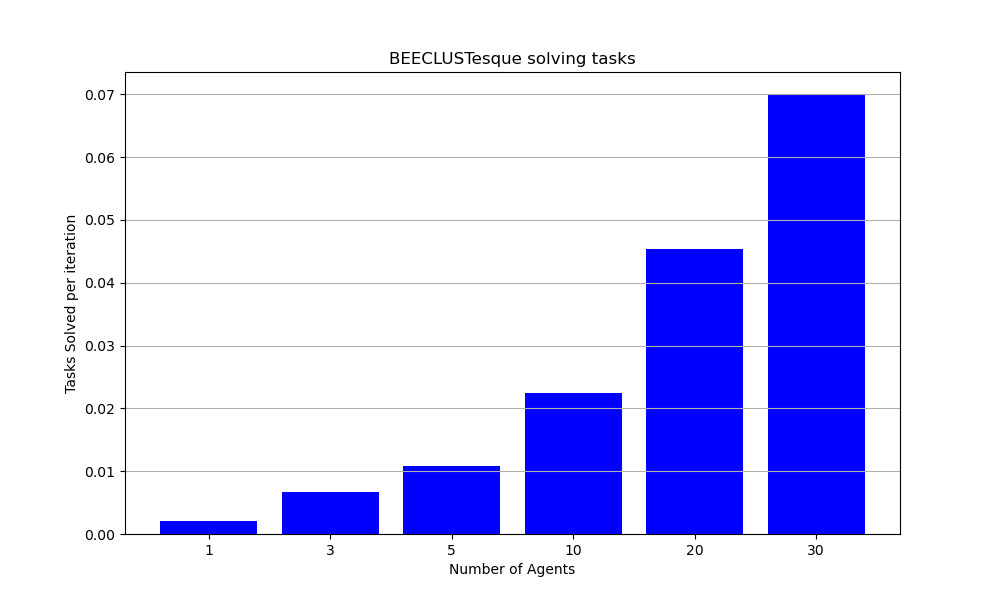
\includegraphics[width=\textwidth]{1_capacity.png}
	\caption{1 agent needed to solve a task, 100000 iterations}
	\label{fig:environment}
\end{figure}

\section{}
See figure 2.
\begin{figure}
	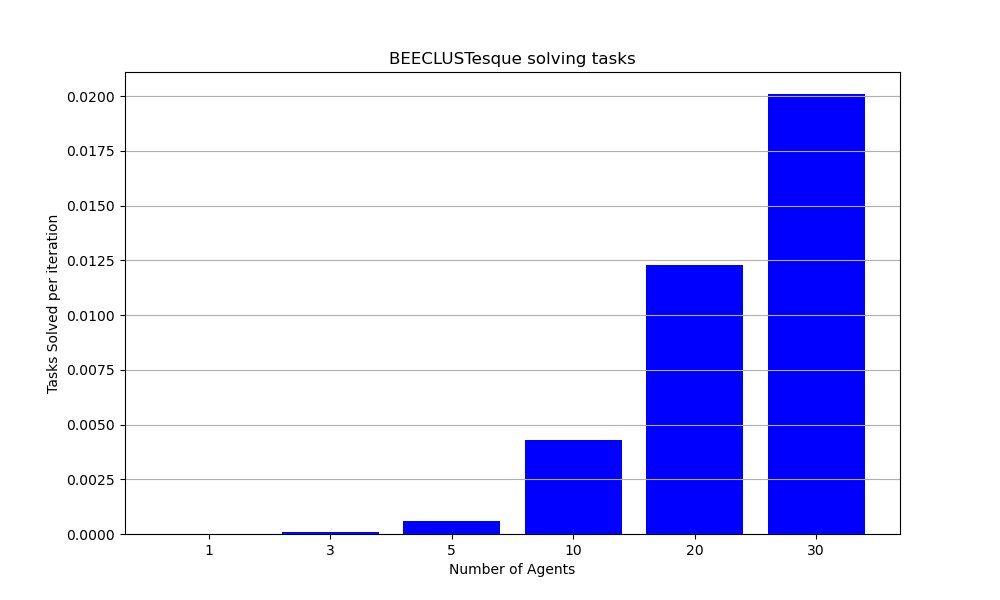
\includegraphics[width=\textwidth]{3_capacity.png}
	\caption{3 agents needed to solve a task, 100000 iterations}
	\label{fig:environment}
\end{figure}
\section{}
In the case of significantly more agents active than how many are needed to solve tasks we get to steady state very quickly as nearly every agent will be on the move at any given time. Especially with $T_c = 1$ we are immediately in steady state as no agent will ever wait.

In the case of higher $T_c$ and more tasks we reach a steady state later. We can consider the average performance of a system to be its performance over e.g. 1000 iterations after reaching steady state, many enough iterations so stochasticity from just a few iterations doesn't impact the average performance a lot. Through trial and error I found 10000 iterations wasn't always enough to get consistent output, so I went with 100000 instead.


\section{}
See figure 3.
\begin{figure}
	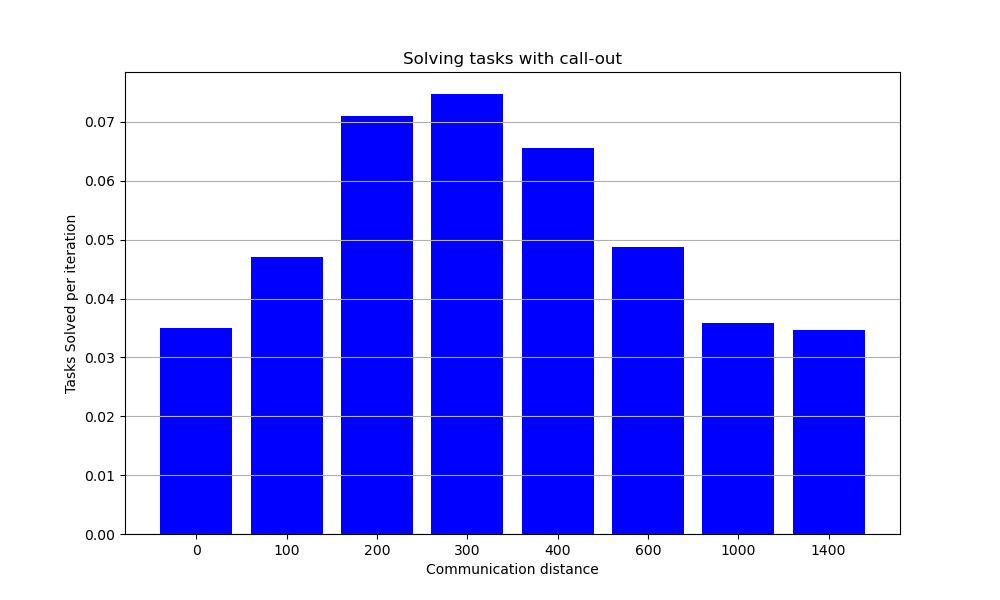
\includegraphics[width=\textwidth]{search_ranges.png}
	\caption{3 agents needed to solve a task, 10000 iterations, 2 tasks}
	\label{fig:environment}
\end{figure}


\appendix

\section{Agent and task classes}
\lstinputlisting[language=Python]{agent.py}


\section{Simulation code}
\lstinputlisting[language=Python]{main.py}

\bibliography{ref}{}
\bibliographystyle{unsrt}
\end{document}

